\chapter{Implementazione\label{sec:implementazione}}
In questa sezione verranno descritte tutte le tecnologie utilizzate per lo sviluppo dell'applicazione.
\section{Ambiente di sviluppo\label{sec:ambiente}}
Per lo sviluppo dell'applicazione è stato utilizzato il sistema di controllo di versione Git,  la realizzazione del progetto è stata eseguita da i seguenti calcolatori:
\begin{itemize}
	\item OS: Windows 10 Home 64bit , Ubuntu 18.04, MacOS Catalina
	\item IDE: Microsoft Visual Studio Code, Android Studio, XCode
\end{itemize}

I dispositivi mobile utilizzati per sviluppo e il test dell'applicazione sono i seguenti:
\begin{itemize}
    \item Acer T04 con Android 6.0 Marshmallow
    \item Xiaomi Mi 9T con Android 9.1 Pie
    \item iPhone XR con iOS (fornito dal dipartimento)
\end{itemize}

\section{Tecnologie usate\label{sec:tecnologie}}
Le tecnologie alle quali ci siamo appoggiati per lo sviluppo dell'applicazione sono:
\begin{description}
    \item[framework Flutter] è un framework cross platform di Google, lo descriviamo meglio in seguito;
    \item[Firebase] platform as a service gestita da Google, fornisce funzionalità di analisi del comportamento degli utenti, memorizzazione di dati, gestione dei login e altro;
    \item[SQLite] DBMS molto leggero per la gestione di basi di dati relazionali.   
\end{description}


\section{Il framework Flutter\label{sec:flutter}}
\subsection{Descrizione\label{sec:flutter-descrizione}}
Flutter è un framework cross-platform cross-compiled realizzato da Google, permette di realizzare applicazioni native eseguibili sia su Android che su iOS realizzando un singolo progetto in linguaggio Dart. La principale caratteristica di Flutter è che l'interfaccia utente è composta unicamente da componenti Widget immutabili. I widget possono definire elementi strutturali (barre, pulsanti, menù), stilistici (font, colori) o di layout (padding), e così via; in pratica ``tutto è un Widget''. Possono essere StatefulWidget, ovvero possedere uno stato ed essere quindi in grado di rispondere alle interazioni dell'utente, oppure StatelessWidget ovvero elementi statici.

Flutter è realizzato in C, C++, Dart e Skia (motore grafico). Le componenti vengono definite in Dart e renderizzate grazie ad un motore implementato in C++ che utilizza le librerie grafiche Skia. Il codice Dart viene compilato in codice nativo utilizzando la compilazione AOT (ahead-of-time) e viene eseguito grazie alla Dart Virtual machine. Il motore C/C++ invece viene compilato con NDK Android o con LLVM (Low Level Virtual Machine) in iOS, permettendo la compilazione in codice nativo \parencite{flutter:presentazione}.

\begin{figure}[htp]
	\centering
	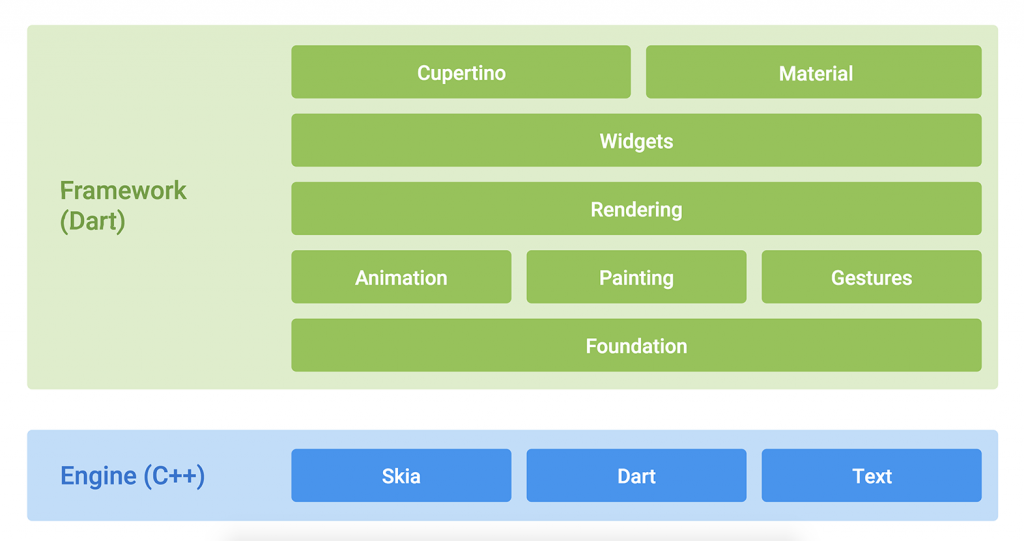
\includegraphics[width=\linewidth]{./immagini/flutter_architecture.png}
	\caption{Architettura di Flutter}
\end{figure}

\subsection{Vantaggi e svantaggi\label{sec:flutter-vantaggi}}
I principali vantaggi che il framework Flutter possiede sono:

\begin{description}
    \item[hot reload] consente di vedere e testare rapidamente i cambiamenti eseguiti sul codice mentre l'applicazione è in esecuzione, quindi rende lo sviluppo veloce;
    \item[widgets] possono essere utilizzati facilmente e sono definiti in stile Material design e Cupertino, permettono quindi la realizzazione di un interfaccia espressiva e flessibile e la loro riusabilità rende lo sviluppo più rapido;
    \item[performance native] il framework essendo cross-compiled garantisce performance al livello di app native;
    \item[documentazione] Flutter è ben documentato e possiede una community di utilizzatori attiva, inoltre è facilmente integrabile con Google Firebase il quale fornisce una rapida implementazione per l'archiviazione dei dati dell'applicazione e delle funzionalità di autenticazione degli utenti;
    \item[ide] sono disponibili vari plugin per il supporto in diversi IDE.
\end{description}

\subsection{Problemi riscontrati e soluzioni apportate}
%Qui siamo sicuri che è giusto parlare di gerarchia?
Durante lo sviluppo dell'applicazione abbiamo riscontrato alcuni problemi legati alle performance dell'applicazione, che non ci soddisfacevano specie dal punto di vista delle animazioni.
Un punto cruciale è la gestione dello stato nella gerarchia dei Widget: per fare in modo che l'applicazione abbia una resa grafica fluida è bene evitare il più possibile l'uso dei Widget stateful \parencite{flutter:performance}.

Inizialmente abbiamo cercato di applicare design pattern noti per esperienze pregresse in modo inappropriato, ad esempio la dependency injection.
Nelle app realizzate con Flutter è sbagliato realizzare le classi alte della gerarchia dei widget con uno stato e fare dependency injection sui widget figli, perché nel momento in cui lo stato di un widget genitore viene modificato, tutti i widget discendenti vengono ridisegnati, in particolar modo viene rieseguito il metodo build.
Nel nostro caso avevamo implementato la schermata principale con uno stato formato da poche variabili che servivano per capire se un utente avesse mai eseguito l'accesso tramite il proprio account Google all'applicazione in precedenza oppure no e per conservarne alcuni dati di utilità.
Queste variabili venivano in seguito iniettate nei widget discendenti per fornire le informazioni necessarie e renderli stateless.

Per risolvere il problema abbiamo deciso di sfruttare pesantemente l'architettura asincrona di Flutter e di eliminare completamente lo stato dove possibile.
Usando in modo opportuno i FutureBuilder, oggetti appositi per gestire l'asincronia nel metodo build (che viene invocato per costruire l'interfaccia), abbiamo ottenuto una resa molto più fluida.

Nei widget in cui non è stato possibile eliminare lo stato, abbiamo comunque fatto in modo di spostarlo il più in basso possibile nella gerarchia, di modo da mantenere delle buone performance.

Un altro problema è stata la gestione dei dati relativi ai voti degli utenti.
Inizialmente abbiamo salvato direttamente i dati collegandoci a Firestore, un servizio offerto da Firebase per la gestione di database con una struttura dinamica orientata ai documenti.
In questo caso però l'utente era costretto a eseguire il login con il proprio account Google per conoscere e salvare i punti guadagnati e il livello di esperienza raggiunto.

La soluzione in questo caso è stata quella di implementare un database locale con una struttura che emula quella del database su Firestore, ma in una versione relazionale, memorizzata attraverso l'uso di SQLite.

\subsection{Comparazione con altri framework\label{sec:flutter-comparazione}}
%TODO intravisto?
Prima di usare Flutter avevamo valutato di usare un framework cross platform intravisto a lezione chiamato Appcelerator Titanium.
Pur essendo un framework adatto allo sviluppo di un'app come Trains, ci sono stati diversi punti a sfavore che ci hanno portato a scegliere Flutter.
Appcelerator Titanium è un framework di tipo interpretato, permette di ottenere app cross platform partendo da codice JavaScript \parencite{gaggi:framework}.
È presente un interprete che consente di ottenere l'app con LAF nativo su Android e iOS.
Pur essendo un framework con cui è possibile ottenere delle ottime performance (basso consumo di risorse e di batteria), ha un grosso punto debole relativo alla documentazione.

A un primo sguardo è presente molta documentazione relativa al framework, ma una volta che si inizia a usare ci si accorge che è molto sparsa e non ben organizzata.
Appcelerator in particolare presenta diverse componenti, non solamente Titanium, che sono necessarie per l'implementazione di app con componenti lato server (database o altro) o per altre funzionalità (ad esempio Alloy è un framework MVC usabile con Titanium che permette di scrivere codice in modo più efficiente e ben organizzato).
Il problema è che la documentazione di tutte le componenti è suddivisa in più siti, a volte è dispersiva, altre volte è presente in uno solo dei vari siti disponibili.

Un altro punto dolente è la quasi totale assenza di tutorial, che rende molto difficile un primo approccio al framework.

Infine i plugin che sono stati sviluppati per il framework non sempre sono completi, ad esempio quelli per l'integrazione con Firebase non lo erano, per cui è stato scelto Flutter, che al contrario dispone di una documentazione ben organizzata, di esempi e tutorial e di plugin funzionanti.